%
%	LaTeX - SCHABLONE fuer die VORTRAGSPRÄSENTATION
%
%	\documentclass[hidesubsections,inrow]{beamer}
\documentclass[hidesubsections,compress]{beamer}
%
% What to output:
%       [notes], [notesonly], [trans], [handout]
% Font family, size selection:
%       [sans], [serif], [mathsans], [mathserif]
%       {smaller,bigger}
% General color trend:
%       {red,blue,grey,brown}
% Topology options:
%       {hide,shade}subsections compress
%       slides{centered,top}

%usepackage{beamerthemesidebardarktab}
%	\usepackage{beamertemplates}		%% no longer supported
%\usepackage[latin1]{inputenc}
%\usepackage[german]{babel}


\usepackage[utf8]{inputenc}
\usepackage[ngerman]{babel}


\usepackage{amsmath,amssymb}
\usepackage{graphicx}
\usepackage{textcomp}
\usepackage{hyperref}
\usepackage{listings}
\usepackage{caption}
\usepackage{subcaption}
\usepackage{multimedia}
\usepackage{pdfpcnotes}
\usepackage{sansmathaccent}
\pdfmapfile{+sansmathaccent.map}


\usetheme{Singapore}
%\usecolortheme{beetle}
\usefonttheme[onlysmall]{structurebold}

\newcommand\lvtyp{SEMINAR}
\newcommand\lvname{Rechnersehen}
\newcommand\lvinst{Computervision Group · FSU Jena}

%
%	HIER WERDEN TITEL REFERENT UND DATUM EINGETRAGEN
%
\newcommand\svthema{3D-Deskriptoren für Aufgaben der Rekonstruktion und Objekterkennung}
\newcommand\svperson{Christian Lengert}
\newcommand\svdatum{20.~Juni 2017}

\title{ \textbf{\textcolor{blue}{\svthema}} }
\author{ \emph{\textcolor{red}{\svperson}} }
\institute{ {\lvtyp} \emph{"`\lvname"'} }
\date{ \tiny \lvinst \\ \svdatum }

\setcounter{tocdepth}{2}
\begin{document}
   \frame { \titlepage }

   \frame{
      \frametitle{Vortragsgliederung}
      \begin{small}
	     \tableofcontents%[subsectionstyle=hide]
      \end{small}
   }
   \section {Einführung}
\frame{ \tableofcontents[currentsection] }
%!TEX root = ../../main.tex
\frame{
\frametitle{3D-Deskriptor?}
	\setbeamertemplate{description item}[align left]
	\begin{description}
		\item[Eingabe] Tiefeninformationsgewinnug $\rightarrow$ \textbf{3D-Punktwolke}
		\item[Verarbeitung] Berechnung, welche Punkt und seine Nachbarschaft betrachtet.
		\item[Ausgabe] Möglichst eindeutige Beschreibung
	\end{description}

	    \begin{figure}
        \centering
        \begin{subfigure}[b]{0.3\textwidth}
            
\includegraphics[width=\textwidth]{topics/intro/n2d.png}
            \caption{2D-Nachbarschaft}
            \label{fig:2dn}
        \end{subfigure}
        ~~~
        \begin{subfigure}[b]{0.3\textwidth}
            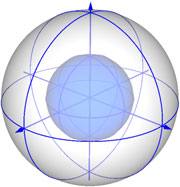
\includegraphics[width=\textwidth]{topics/intro/n3d.png}
            \caption{3D-Nachbarschaft}
            \label{fig:3dn}
        \end{subfigure}
    \end{figure}


}

\subsection{Objekterkennung}
\frame{
	\frametitle{Objekterkennung}
	Finde bekanntes Objekt in einer Szene:
	\begin{enumerate}
		\item Berechne Deskriptoren für Modell
		\item Berechne Deskriptoren für Szene
		\item Vergleiche berechnete Deskriptoren
	\end{enumerate}


		 \begin{figure}
        \centering
        \begin{subfigure}[b]{0.45\textwidth}
            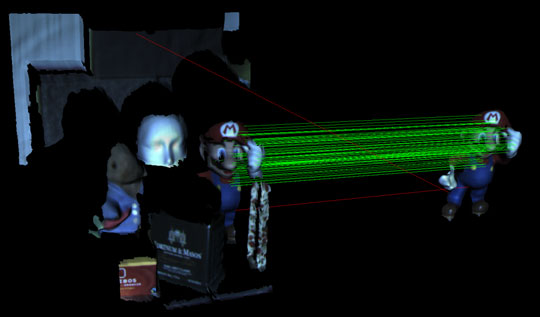
\includegraphics[width=\textwidth]{topics/intro/matchingScene.png}
            \caption{Finde Objekt}
            \label{fig:find}
        \end{subfigure}
        ~~~
        \begin{subfigure}[b]{0.45\textwidth}
           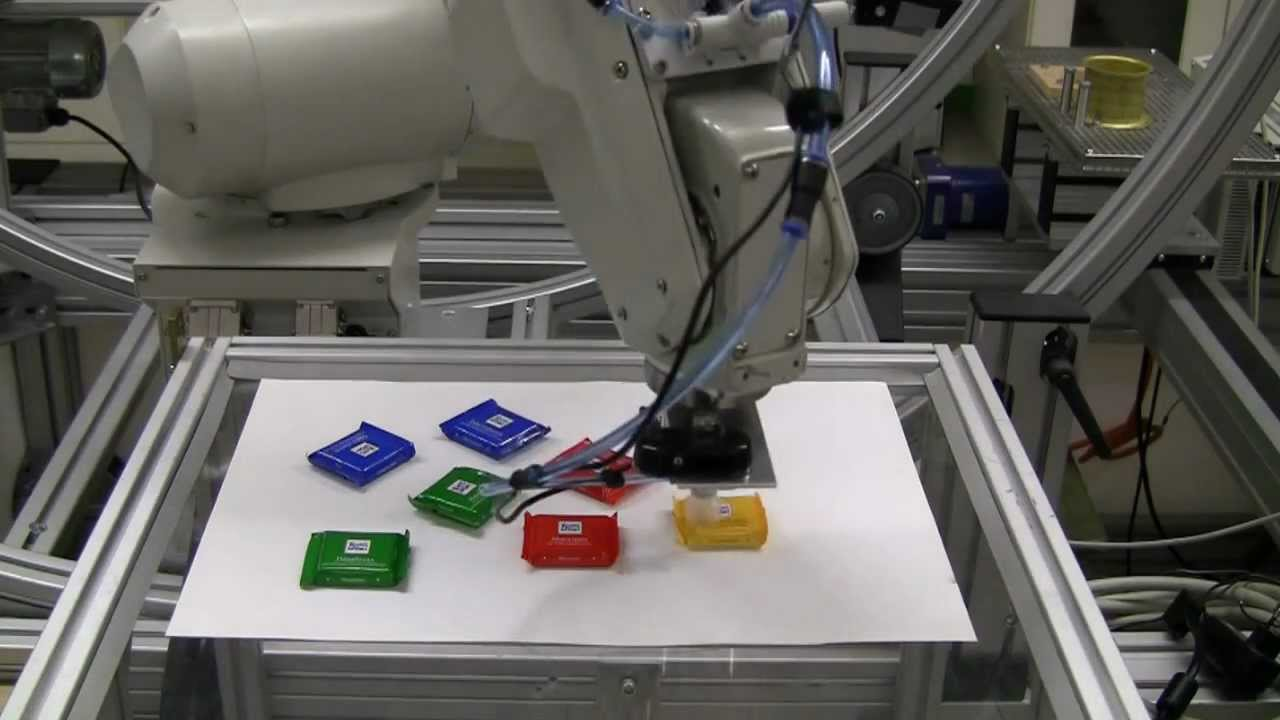
\includegraphics[width=\textwidth]{topics/intro/objRec1.jpg}
            \caption{Bestimme Lage.}
            \label{fig:3dn}
        \end{subfigure}
    \end{figure}

	\centering
		
}

\subsection{Rekonstruktion}
\frame{
	\frametitle{Rekonstruktion}

\begin{flushleft}
\setbeamertemplate{description item}[align left]
            \begin{description}
            	\item[Genauigkeit] von verwendeten Verfahren nicht ausreichend.
            	\item[Textur] ist von entscheidender Bedeutung
            	\item[Interpolation] von gewonnenen Bildpunkten.
            	\item[Besseres] Modell der Umgebung
			\end{description}

		\begin{itemize}
			\item Automatisierte Baumaschinen
			\item Automatische Landung von Raumsonden
		\end{itemize}
\end{flushleft}

\setbeamertemplate{description item}[align left]
            \begin{description}
            	\item[Daten] von mehreren Sensoren/Verfahren.
            	\item[Kombination] zu einer einzigen Punktwolke
			\end{description}

}
\section{Einsatzbereiche}
\frame{\tableofcontents[currentsection]}
%!TEX root = ../../main.tex


\subsection{Struktur}
\frame{
	\frametitle{Was gehört dazu?}

	\begin{description}
		\item [Feature Selection] Welche Punkte sind \textit{repräsentativ} für das Objekt/die Szene?
		\item [1. Reference Frame/Axis] Welche \textit{Referenz} wird für die Nachbarschaft gewählt
		\item [2. Histogramm/Signatur] Welche \textit{Berechnungsvorschrift} wird ausgeführt?
		\item [3. Matching-Phase] Wie werden berechnete Deskriptoren verglichen?
	\end{description}


	    \begin{figure}
        \centering
        \begin{subfigure}[b]{0.35\textwidth}
            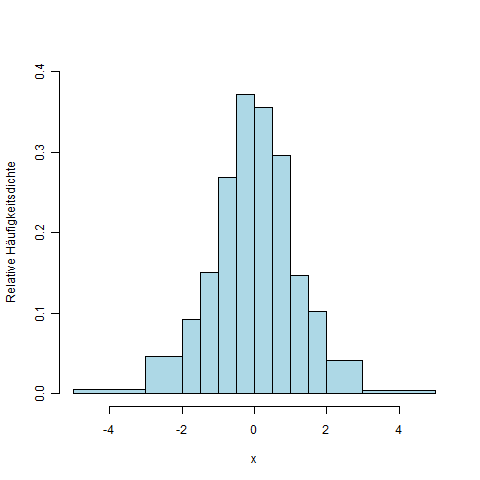
\includegraphics[width=\textwidth]{topics/eigenschaften/hist.png}
            \caption{Histogramm}
            \label{fig:hist}
        \end{subfigure}
        ~~~
        \begin{subfigure}[b]{0.35\textwidth}
            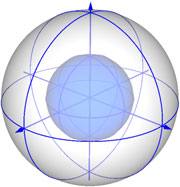
\includegraphics[width=\textwidth]{topics/intro/n3d.png}
            \caption{3D-Nachbarschaft}
            \label{fig:ctKnut}
        \end{subfigure}
    \end{figure}


}
\subsection{Schwierigkeiten}
\frame{
	\frametitle{Was sind die Schwierigkeiten?}

	\begin{flushleft}
	\setbeamertemplate{description item}[align left]
	\begin{description}
		\item[Geometrische Transformationen] Rotation und Translation sollen möglichst geringen Einfluss auf das Ergebnis haben.
		\item[Skalierung] Ein in der größe skaliertes Objekt soll die selbe Deskription erhalten.
		\item[Punktdichte] Unterschiedliche Sensoren und Blickwinkel führen zu Schwankungen.
		\item[Clutter] Viele Objekte, ein Durcheinander
		\item[Verdeckung] Objekte verdecken andere
		\item[Vorzeichen] Eindeutigkeit des Referenzsystems.
	\end{description}
	\end{flushleft}
}
\section{Auswahl}
\frame{ \tableofcontents[currentsection] }
%!TEX root = ../../main.tex
\subsection{Spin Images}
\frame{
	\frametitle{Spin Images (1999) Johnson \& Herbert}
%	\begin{description}
%		\item[Berechnungsvorschrift] rotiere \textbf{Histogramm} um Referenzachse
%	\end{description}
		\begin{itemize}
		\item Berechne Oberflächennormale im Zielpunkt $\rightarrow$ Referenzachse
		\item Spanne Zylinder $z=(r,h)$ um RA auf
		\item rotiere \textbf{Histogramm} um RA
		\item Zähle Punkte auf ``Umlaufbahn'' $(r,h)$ $\rightarrow$ Spin-Image
		\item Wähle dabei nur Punkte, deren Normale maximal einen gewählten Winkel von der Punktnormale abweicht
	\end{itemize}
	\centering
		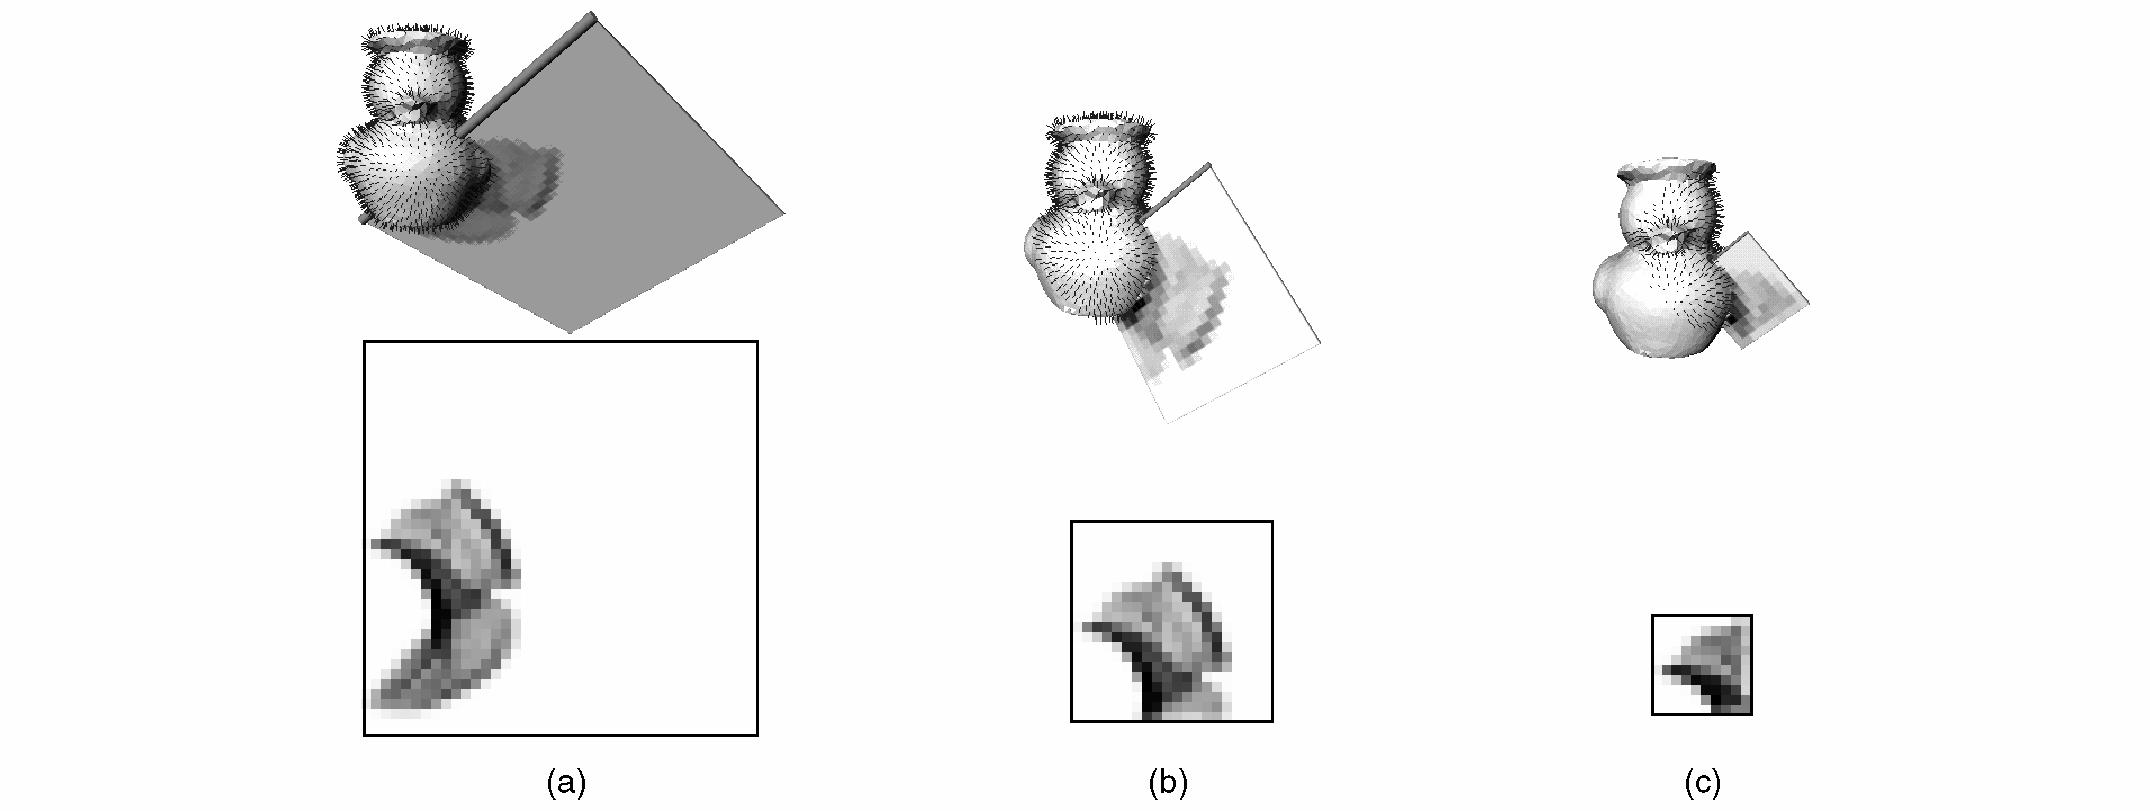
\includegraphics[width=\textwidth]{topics/auswahl/spinImages/si1.jpg}

}

\frame{
	\frametitle{Spin Images (1999) Johnson \& Herbert}
	\begin{flushleft}
	\setbeamertemplate{description item}[align left]
	\begin{description}
		\item[Parameter] Zylinderradius und -höhe, Normalenschwellenwert, Histogrammauflösung
	\item[Referenz] 
		\begin{itemize}
			\item Referenzachse in Punktnormale
			\item Nicht eindeutig aufgrund des Vorzeichens
		\end{itemize}
	\item[Berechnugsmethode] Histogramm
	\item[Vergleich] Korrelation
    \end{description}
    \end{flushleft}
    \centering
		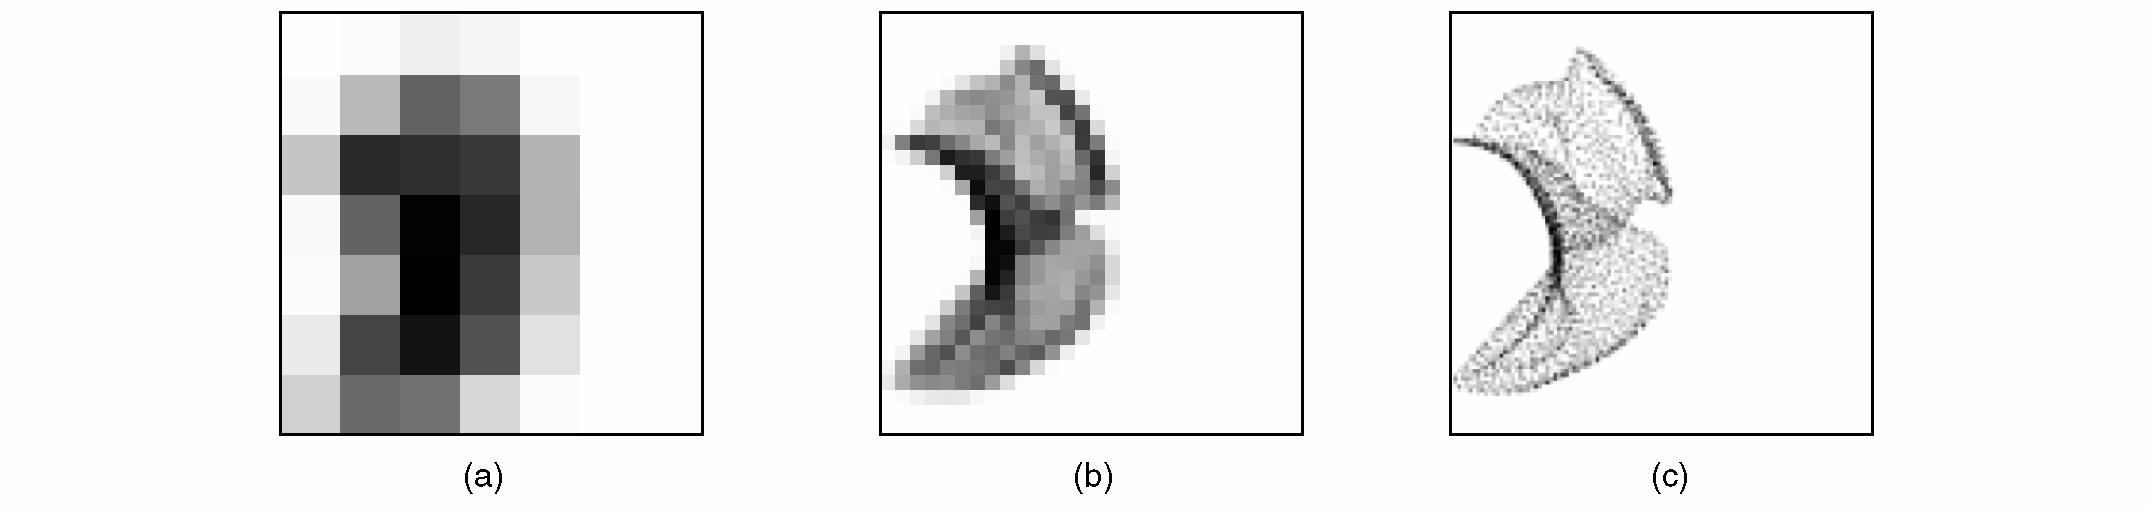
\includegraphics[width=\textwidth]{topics/auswahl/spinImages/si2.jpg}
}	



\subsection{Point Signatures}
\frame{
	\frametitle{Point Signatures (1996)  Chua \& Jarvis}

			\begin{itemize}
		\item Berechne Oberflächennormale im Zielpunkt $p$ $\rightarrow$ $N$
		\item Lege Sphäre mit Radius $r$ um $p$
		\item Schneide Sphäre mit Oberfläche $\rightarrow$ 3D-Kurve $C$
		\item Approximiere tangentiale Ebene an $p$ $\rightarrow$ $P'$
		\item Projiziere $C$ auf $P'$  $\rightarrow$ planare Kurve $C'$
		\item Wähle Referenzwinkel $\Theta_0$ nach dem höchsten Wert in $C'$

	\end{itemize}

	\centering
		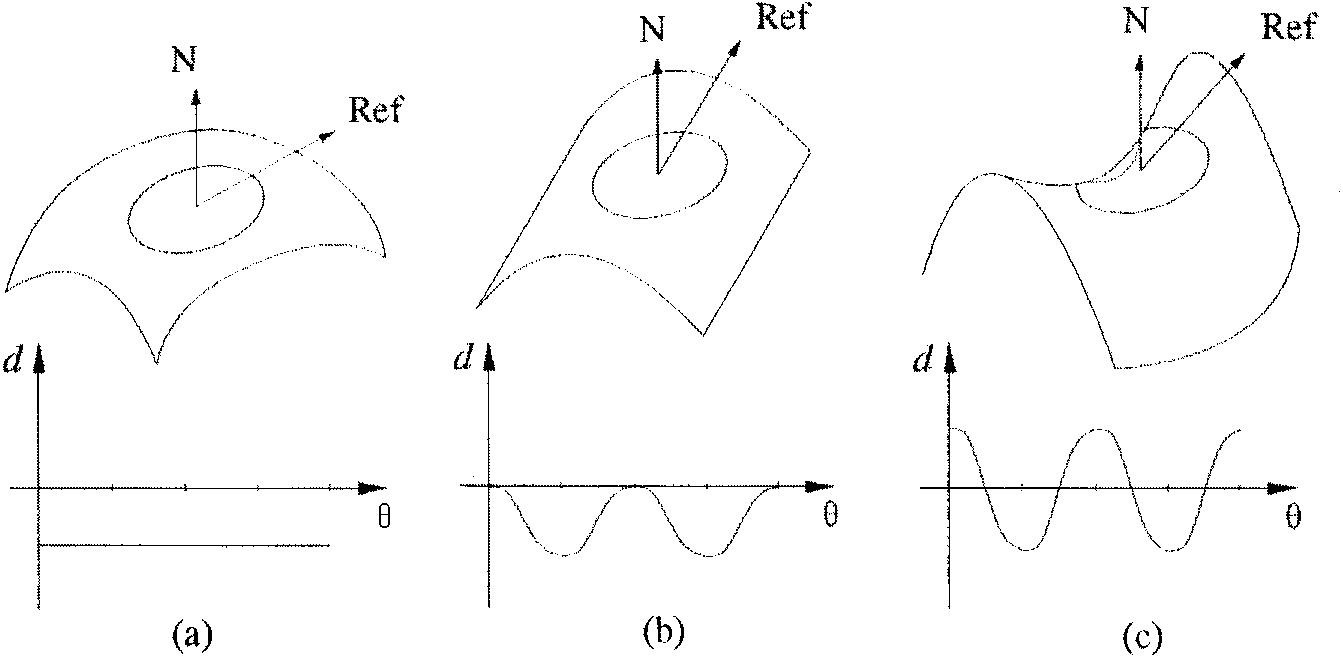
\includegraphics[width=0.8\textwidth]{topics/auswahl/pointSignatures/ps.jpg}
}

\frame{
	\frametitle{Point Signatures (1996)  Chua \& Jarvis}
	\begin{flushleft}
	\setbeamertemplate{description item}[align left]
	\begin{description}
		\item[Parameter] Sphärenradius, Schwellenwert
	\item[Referenz] 
		\begin{itemize}
			\item Referenzrahmen, Normale und Startwinkel, Anzahl der Skalen
			\item Variant gegenüber Skalierung, da fester Radius $\rightarrow$ berechne mit mehreren Radien pro Modell
		\end{itemize}
	\item[Berechnugsmethode] Signatur
	\item[Vergleich] $|d_1(\Theta_i)-d_2(\Theta_i) > \epsilon|$


    \end{description}
    \end{flushleft}

    \centering
		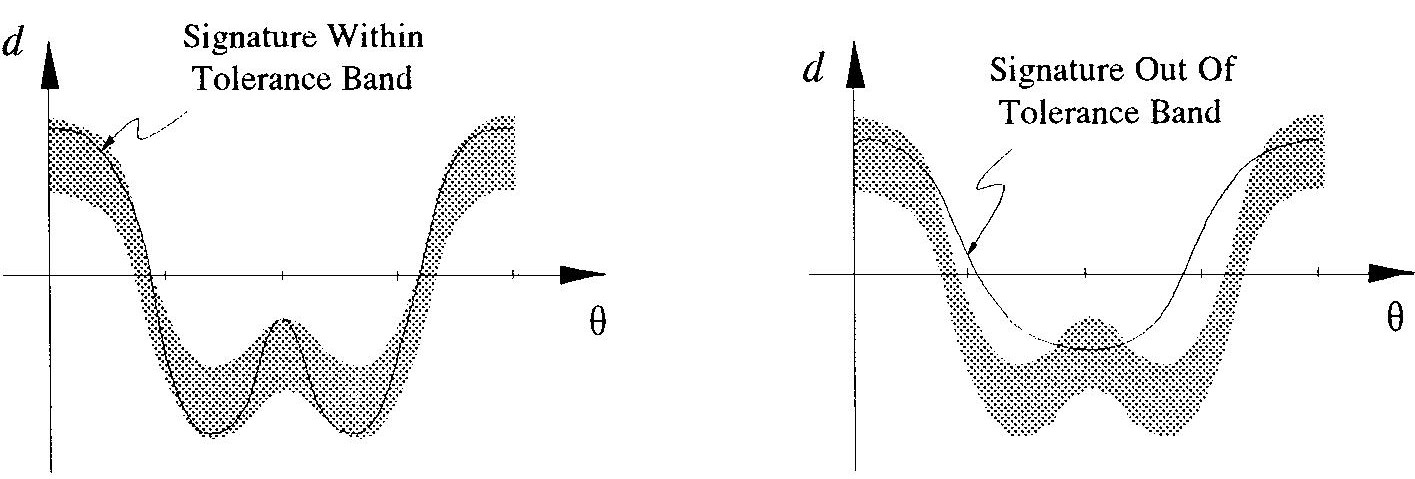
\includegraphics[width=0.8\textwidth]{topics/auswahl/pointSignatures/m.jpg}
}




\subsection{Exponential Mapping}
\frame{
	\frametitle{Exponential Mapping (2008) Novatnack \& Nishino}

			\begin{itemize}
		\item Wähle eine sphärische Nachbarschaft mit Radius $\sigma$ für den Zielpunkt $p$
		\item Berechne für jeden Nachbarn die geodätischen Koordinaten $\mathbb{G}(u,v)=(d_g(u,v),\Theta_\tau(u,v))$
		\item Fasse die für jeden Nachbarn berechneten Tupel als skalenabhänigen Deskriptor $mathbb{G}^\sigma_p$zusammen.
		\item Berechne $\mathbb{G}^\sigma_p$ für mehrere $\sigma$ pro Punkt um skalenunabhängigen Deskriptor zu erzeugen.


	\end{itemize}

    \centering
		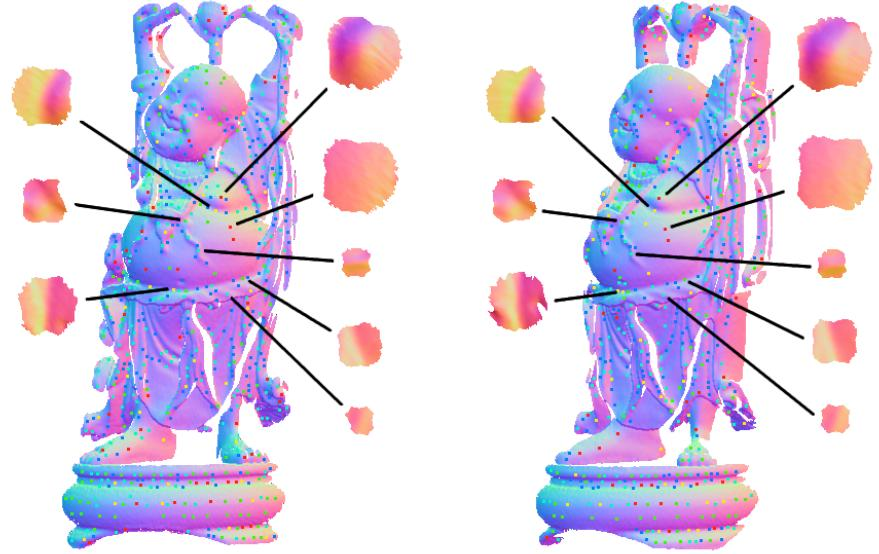
\includegraphics[width=0.4\textwidth]{topics/auswahl/exponentialMapping/em1.jpg}
}

\subsection{Exponential Mapping}
\frame{
	\frametitle{Exponential Mapping (2008) Novatnack \& Nishino}

	\begin{flushleft}
	\setbeamertemplate{description item}[align left]
	\begin{description}
		\item[Parameter] Anzahl der Skalen, Sphärenradien
	\item[Referenz] 
		\begin{itemize}
			\item Referenzrahmen
			\item Variant gegenüber Skalierung, da fester Radius $\rightarrow$ berechne mit mehreren Radien pro Modell
		\end{itemize}
	\item[Berechnugsmethode] Signatur
	\item[Vergleich] Normalisierte Kreuzkorrelation
\end{description}
    \end{flushleft}

        \centering
		
\includegraphics[width=0.4\textwidth]{topics/auswahl/exponentialMapping/em2.jpg}
}

\subsection{SHOT}
\frame{
	\frametitle{Signatures of Histogramms of Orientations}
	SHOT (2010) Tombari, Salti \& Stefano

	
}

\frame{
	\frametitle{SHOT (2010) Tombari, Salti \& Stefano}
}
\section{Vergleich}
\frame{ \tableofcontents[currentsection] }
%!TEX root = ../../main.tex
\frame{
	\frametitle{Im Experiment}
	\begin{description}
		\item[Feature Points per Model] 1000
	\end{description}
	\centering
		\textbf{Versuch 1}~~~~~~~~~~~~~\textbf{Versuch 2}~~~~~~~~~~~~~\textbf{Versuch 3}
		\begin{columns}[t]
	 	
    	\begin{column}{4cm}
    	\centering


    	\begin{itemize}
    		\item 6 Modelle aus Stanford 3D Scanning Repository
    		\item Mit jeweils einigen Modellen 45 Szenen erzeugt
    		\item 45 Szenen mit Gaussrauschen versetzt $(\sigma \in {0.1,0.2,0.3})$.
    	\end{itemize} 

     	\end{column}
    	\begin{column}{4cm}
    	\centering
    	\begin{itemize}
    		\item Szenen aus Versuch 1
    		\item Subsampling $f = \frac{1}{8}$
    		
    	\end{itemize} 
    	\end{column}
    	\begin{column}{4cm}
    	\begin{itemize}
    	    			\item 8 Modelle, im Labor erzeugt mit Spacetime-Stereo.
    			\item 15 Szenen, die jeweils zwei der acht Objekte enthalten.	
    		\end{itemize}  
    	
    	\end{column}
    \end{columns}

}


\subsection{Bewertung}
\frame{
	\frametitle{False-Posives?}
	\centering
		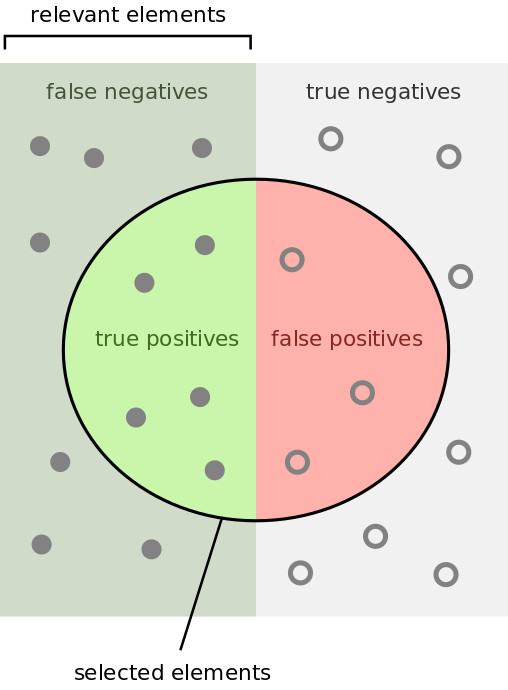
\includegraphics[height=0.8\textheight]{topics/vergleich/pr.jpg}
}

%%Precision recall
\frame{
	\frametitle{Die Maße: Precision und Recall}
	\begin{columns}[c]
    	\begin{column}{5cm}
     		Wie viele der gelieferten Muster sind relevant?
     		$$Precision = \frac{|TP|}{|TP|+|FP|}$$
     		Wie viele der richtigen Muster wurden geliefert? 
     		$$ Recall\frac{|TP|}{|TP|+|FN|}$$
     	\end{column}
    	\begin{column}{5cm}
     		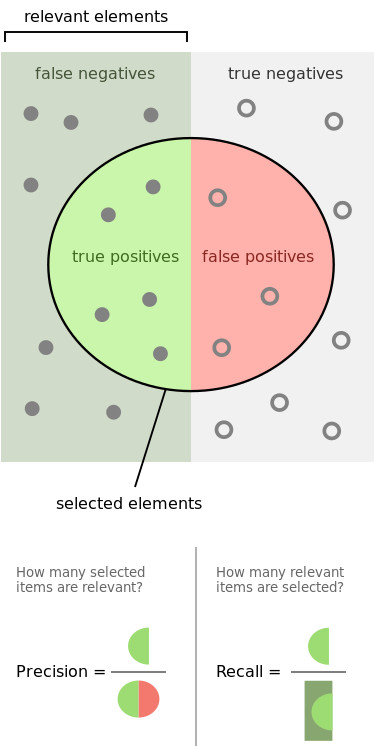
\includegraphics[height=0.8\textheight]{topics/vergleich/pr2.jpg}
    	\end{column}
    \end{columns}
}


\subsection{Ergebnisse}
\frame{
	\frametitle{Ergebnis: Versuch 1}
	\centering
	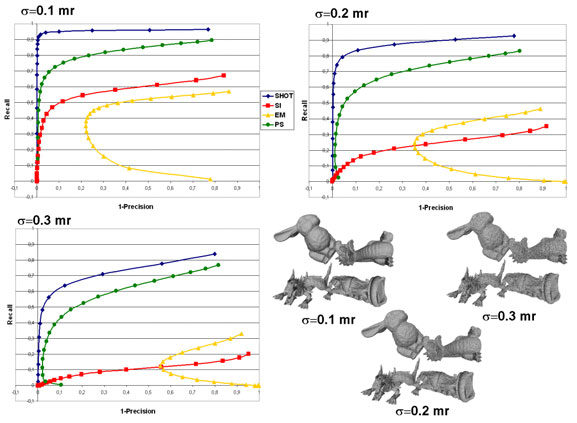
\includegraphics[height=0.8\textheight]{topics/vergleich/v1.png}
}

\frame{
	\frametitle{Ergebnis: Versuch 2}
	\centering
	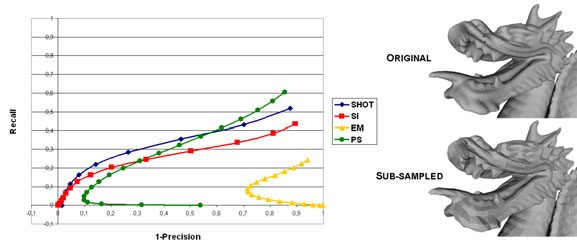
\includegraphics[width=\textwidth]{topics/vergleich/subSampled.png}
}

\frame{
	\frametitle{Ergebnis: Versuch 3}
	\centering
	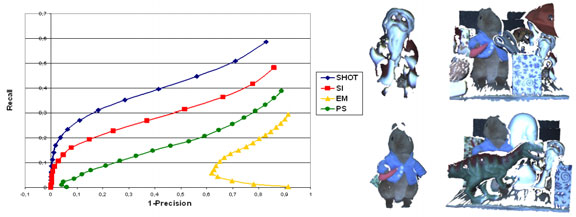
\includegraphics[width=\textwidth]{topics/vergleich/v3.png}
}
\frame{\frametitle{Vielen Dank für die 
Aufmerksamkeit}}
\end{document}
